
\documentclass[10 pt,usenames,dvipsnames, oneside]{article}
\usepackage{../../../modelo-fracoes}
\graphicspath{{../../../Figuras/licao02/}}


\begin{document}

\begin{center}
  \begin{minipage}[l]{3cm}

\includegraphics[width=2cm]{logo}    
\end{minipage}\hfill
\begin{minipage}[r]{.8\textwidth}
 {\Large \scshape Atividade: Corrida de carrinhos}  
\end{minipage}
\end{center}
\vspace{.2cm}

\ifdefined\prof
\begin{goals}
\begin{enumerate}

    \item       Marcar em uma semirreta pontos cujas distâncias até um ponto de referência são frações do comprimento de um segmento dado.

\end{enumerate}
\tcblower

  \begin{itemize} %s
    \item       Esta é uma atividade que pode ser realizada individualmente.
    \item       Esta é uma atividade preparatória para a representação de frações na reta numérica, assunto da próxima lição.
    \item       Observe que, nesta atividade, as distâncias estão associadas aos segmentos determinados pelos percursos dos carrinhos na pista, e correspondem a frações da distância percorrida pelo carrinho de Lucas, que assume papel de unidade.
      % não se espera precisão, bastam marcações coerentes.
    \item       Não se espera, nem se recomenda, que as marcações feitas pelos alunos na pista sejam feitas com precisão, marcações coerentes são suficientes. Contudo, é preciso ficar atento para que as marcações dos carrinhos de Heitor e de Lorenzo coincidam. A mesma observação se aplica aos carrinhos de Rafael, Samuel e de Guilherme. De fato, três metades do percurso de Lucas coincide com seis quartos do percurso de Lucas.
    \item       Aqui, a definição de fração não unitária como justaposição de frações unitárias pode ser usada para justificar o porquê, por exemplo, de os carrinhos de Rafael e de Samuel terem parado na mesma posição.
    \item       Assim, espera-se que a distância percorrida pelo carrinho de Matheus (item a) seja associada à metade do segmento que identifica a distância percorrida pelo carrinho de Lucas, que corresponde à unidade e está destacado em vermelho na imagem. Já a distância percorrida pelo carrinho de Heitor (item b) deve ser associada à justaposição de       $3$ segmentos correspondentes à distância percorrida pelo carrinho de Matheus. Espera-se que as demais distâncias sejam obtidas de forma semelhante. Cabe destacar, no entanto, que para determinar as distâncias percorridas pelos carrinhos de Lorenzo e de Samuel, será necessário determinar       $\frac{1}{4}$ e       $\frac{1}{3}$ da unidade, respectivamente.
  %  \item       De forma geral, se $d$ é a distância percorrida pelo carrinho de Lucas, então a partição em $2$ partes iguais de um segmento $u$ cujo comprimento é $d$ determina dois segmentos congruentes $s$ e $s'$ que correspondem à $\frac{1}{2}$ de       $u$ e cujos comprimentos são, portanto, iguais a       $\frac{1}{2}$ de       $d$. A justaposição de       $2$ cópias de       $s$ ($\frac{2}{2}$ de       $u$) tem comprimento       $d$ e, sendo assim, a justaposição de       $4$ cópias de       $s$ ($\frac{4}{2}$ de $u$) tem comprimento       $2d$. Do mesmo modo, se       $t$ é um segmento que corresponde à       $\frac{1}{3}$ de       $u$, então a justaposição de       $3$ cópias de       $t$ ($\frac{3}{3}$ de       $u$) tem comprimento       $d$ e, em consequência, a justaposição de       $6$ cópias de $t$ ($\frac{6}{3}$ de $u$) tem comprimento $2d$. Assim, os carrinhos de Rafael e de Samuel percorreram a mesma distância ($2d$) e, como eles saíram do mesmo ponto de largada, suas posições finais são iguais.
\end{itemize} %s

\end{goals}

\bigskip
\begin{center}
{\large \scshape Atividade}
\end{center}
\fi

Lucas, Matheus, Heitor, Rafael, Enzo, Nicolas, Lorenzo, Guilherme e Samuel estavam brincando de empurrar seus carrinhos de brinquedo para ver qual carrinho ia mais longe em uma pista reta.

A figura a seguir mostra o quão longe foi o carrinho de Lucas e onde ele parou na pista com relação ao ponto de largada.

\begin{center}
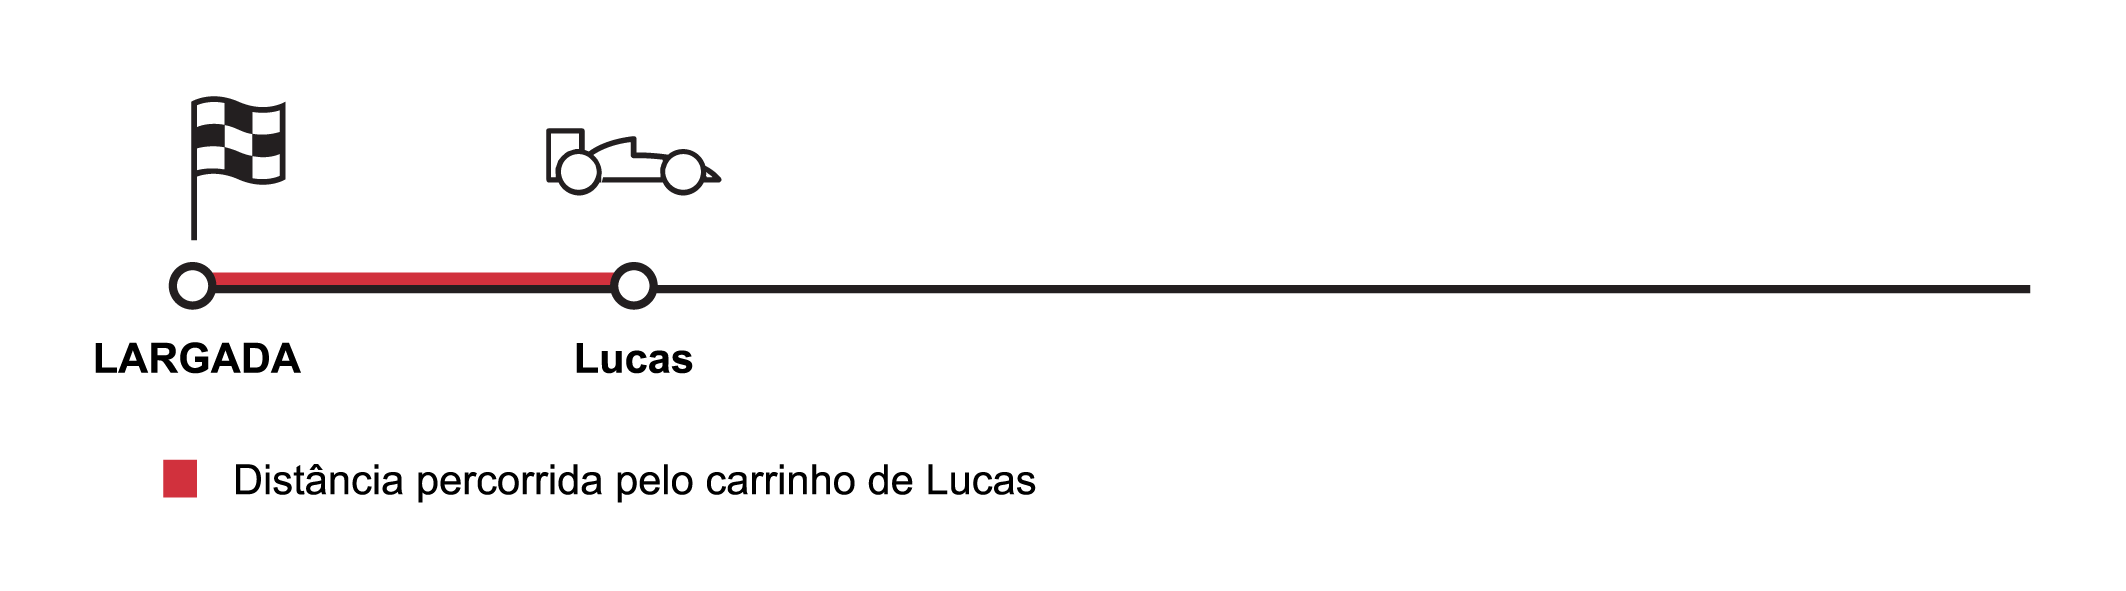
\includegraphics[width=450pt, keepaspectratio]{ativ12_fig01.png}
\end{center}

Sabe-se que:

\begin{enumerate} [label=\alph*)] %s
  \item     O carrinho de Matheus só conseguiu ir até a metade da distância percorrida pelo carrinho de Lucas.
  \item     O carrinho de Heitor conseguiu ir até     $\frac{3}{2}$     da distância percorrida pelo carrinho de Lucas.
  \item     O carrinho de Rafael conseguiu ir até     $\frac{4}{2}$     da distância percorrida pelo carrinho de Lucas.
  \item     O carrinho de Enzo conseguiu ir até     $\frac{5}{2}$     da distância percorrida pelo carrinho de Lucas.
  \item     O carrinho de Nicolas conseguiu ir até     $\frac{6}{2}$     da distância percorrida pelo carrinho de Lucas.
  \item     O carrinho de Lorenzo conseguiu ir até     $\frac{6}{4}$     da distância percorrida pelo carrinho de Lucas.
  \item     O carrinho de Guilherme conseguiu ir até o dobro da distância percorrida pelo carrinho de Lucas.
  \item     O carrinho de Samuel conseguiu ir até     $\frac{6}{3}$     da distância percorrida pelo carrinho de Lucas.
\end{enumerate} %s


Com essas informações, marque as posições de parada dos carrinhos de todos os amigos de Lucas no encarte que você irá receber.

\begin{center}
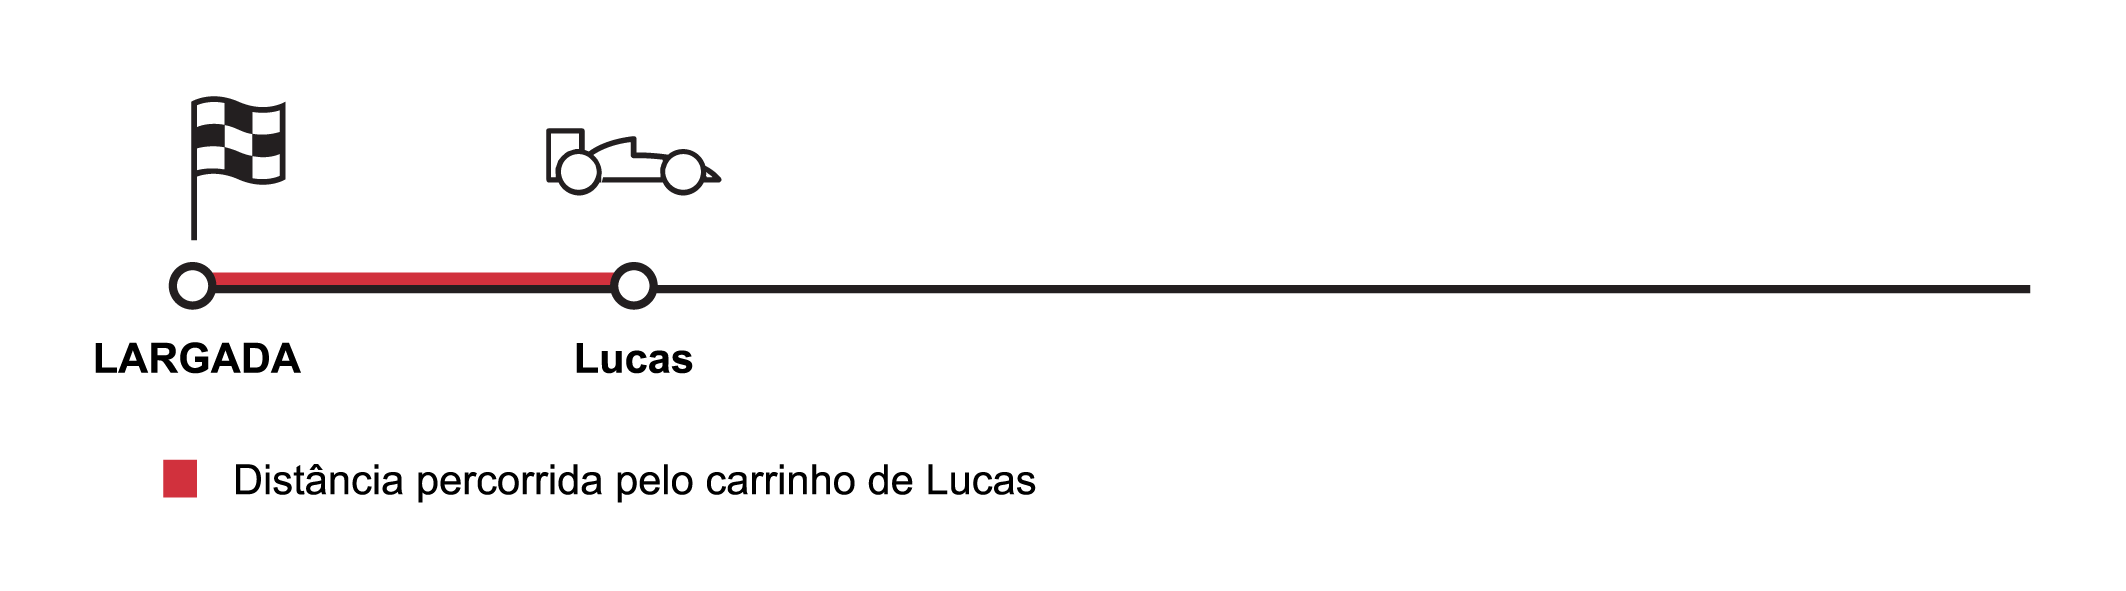
\includegraphics[width=450pt, keepaspectratio]{ativ12_fig01.png}
\end{center}


Os carrinhos de Rafael e Samuel pararam no mesmo lugar? Explique.

\ifdefined\prof

\begin{solucao}


Do item a) sabe-se que o carrinho de Matheus só conseguiu ir até a metade da distância percorrida pelo carrinho de Lucas. 

\hspace{-15mm} 

\begin{center}

\begin{tikzpicture}[]

\tikzstyle{circ}=[draw, circle, inner sep=.075cm, node distance=1.75cm, thick];

\tikzstyle{circ2}=[circle, inner sep=.075cm, node distance=1.75cm, thick];

\node (larg) [circ, label=below:Largada] {} ;

\node (1) [circ, right of=larg, label=below:Matheus] {} node [above of=1, node distance=.5cm]{
\includegraphics[width=1cm]{carrinho2.png}};

\node (2) [circ, right of=1, label=below:Lucas] {} node [above of=2, node distance=.5cm]{
\includegraphics[width=1cm]{carrinho2.png}};

\node (3) [right of=2, circ2] {} ;

\node (4) [right of=3, circ2] {};

\node (5) [right of=4, circ2] {};

\node (6) [right of=5, circ2] {};

\path[thick]

(larg) edge (1)
(1) edge (2)
(2) edge (6)
;
\end{tikzpicture}
\end{center}

  Do item b), o carrinho de Heitor conseguiu ir até $\frac{3}{2}$ da ``distância percorrida pelo carrinho de Lucas'' (a unidade).  Isso permite marcar a posição do carrinho de Heitor justapondo-se 3 metades da unidades a partir do ponto de partida.

  \hspace{-15mm} 

\begin{center}
\begin{tikzpicture}[]

\tikzstyle{circ}=[draw, circle, inner sep=.075cm, node distance=1.75cm, thick];

\tikzstyle{circ2}=[circle, inner sep=.075cm, node distance=1.75cm, thick];

\node (larg) [circ, label=below:Largada] {} ;

\node (1) [circ, right of=larg, label=below:Matheus] {} node [above of=1, node distance=.5cm]{
\includegraphics[width=1cm]{carrinho2.png}};

\node (2) [circ, right of=1, label=below:Lucas] {} node [above of=2, node distance=.5cm]{
\includegraphics[width=1cm]{carrinho2.png}};

\node (3) [circ, right of=2, label=below:Heitor] {} node [above of=3, node distance=.5cm] {
\includegraphics[width=1cm]{carrinho2.png}};

\node (4) [circ2, right of=3] {};

\node (5) [circ2, right of=4] {};

\node (6) [circ2, right of=5] {};

% \node (7) [circ, right of=6, label=below:Guilherme] {} node [above of=7, node distance=.5cm] {
\includegraphics[width=1cm]{carrinho2.png}};

\path[thick]

(larg) edge (1)
(1) edge (2)
(2) edge (3)
(3) edge (6)
% (6) edge (7)
;
\end{tikzpicture}
\end{center}


  Os itens c), d) e e) afirmam que os carrinhos de Rafael, Enzo e Nicolas conseguiram ir até $\frac{4}{2}$, $\frac{5}{2}$ e $\frac{6}{2}$  da distância percorrida pelo carrinho de Lucas, respectivamente. Então pode-se marcar as distâncias percorridas pelos carrinhos de Rafael, Enzo e Nicolas justapondo-se, respectivamente, 4, 5 e 6 meios da unidade.

  \hspace{-15mm} 

\begin{center}
\begin{tikzpicture}[]

\tikzstyle{circ}=[draw, circle, inner sep=.075cm, node distance=1.75cm, thick];

\tikzstyle{circ2}=[circle, inner sep=.075cm, node distance=1.75cm, thick];

\node (larg) [circ, label=below:Largada] {} ;

\node (1) [circ, right of=larg, label=below:Matheus] {} node [above of=1, node distance=.5cm]{
\includegraphics[width=1cm]{carrinho2.png}};

\node (2) [circ, right of=1, label=below:Lucas] {} node [above of=2, node distance=.5cm]{
\includegraphics[width=1cm]{carrinho2.png}};

\node (3) [circ, right of=2, label=below:Heitor] {} node [above of=3, node distance=.5cm] {
\includegraphics[width=1cm]{carrinho2.png}};

\node (4) [circ, right of=3, label=below:Rafael] {} node [above of=4, node distance=.5cm] {
\includegraphics[width=1cm]{carrinho2.png}};

\node (5) [circ, right of=4, label=below:{Enzo}] {} node [above of=5, node distance=.5cm] {
\includegraphics[width=1cm]{carrinho2.png}};

\node (6) [circ, right of=5, label=below:{Nicolas}] {} node [above of=6, node distance=.5cm] {
\includegraphics[width=1cm]{carrinho2.png}};

% \node (7) [circ, right of=6, label=below:Guilherme] {} node [above of=7, node distance=.5cm] {
\includegraphics[width=1cm]{carrinho2.png}};

\path[thick]

(larg) edge (1)
(1) edge (2)
(2) edge (3)
(3) edge (4)
(4) edge (5)
(5) edge (6)
% (6) edge (7)
;
\end{tikzpicture}
\end{center}
  

  Do item f), o carrinho de Lorenzo percorreu $\frac{6}{4}$ da distância percorrida pelo carrinho de Lucas. Para marcar seis quartos dessa unidade, divide-se a distância percorrida por Lucas em quartos e justapõe-se seis partes iguais a essa a partir do ponto de partida.

  Agora surge a dúvida das posições relativas de paradas dos carrinhos de Lorenzo e Heitor. Para isso é importante observar que dois quartos corresponde à metade da distância percorrida pelo carrinho de Lucas e, portanto, que seis quartos corresponde à três metades (três meios) dessa distância. Logo os carrinhos de Lorenzo e Heitor pararam na mesma posição.

  \hspace{-15mm} 

\begin{center}
\begin{tikzpicture}[]

\tikzstyle{circ}=[draw, circle, inner sep=.075cm, node distance=1.75cm, thick];

\node (larg) [circ, label=below:Largada] {} ;

\node (1) [circ, right of=larg, label=below:Matheus] {} node [above of=1, node distance=.5cm]{
\includegraphics[width=1cm]{carrinho2.png}};

\node (2) [circ, right of=1, label=below:Lucas] {} node [above of=2, node distance=.5cm]{
\includegraphics[width=1cm]{carrinho2.png}};

\node (3) [circ, right of=2, label={[below of=4, align=center, node distance=.7cm] Heitor e\\Lorenzo}] {} node [above of=3, node distance=.5cm] {
\includegraphics[width=1cm]{carrinho2.png}};

\node (4) [circ, right of=3, label=below:Rafael] {} node [above of=4, node distance=.5cm] {
\includegraphics[width=1cm]{carrinho2.png}};

\node (5) [circ, right of=4, label=below:{Enzo}] {} node [above of=5, node distance=.5cm] {
\includegraphics[width=1cm]{carrinho2.png}};

\node (6) [circ, right of=5, label=below:{Nicolas}] {} node [above of=6, node distance=.5cm] {
\includegraphics[width=1cm]{carrinho2.png}};

% \node (7) [circ, right of=6, label=below:Guilherme] {} node [above of=7, node distance=.5cm] {
\includegraphics[width=1cm]{carrinho2.png}};

\path[thick]

(larg) edge (1)
(1) edge (2)
(2) edge (3)
(3) edge (4)
(4) edge (5)
(5) edge (6)
% (6) edge (7)
;
\end{tikzpicture}
\end{center}


Do item g), o carrinho de Guilherme percorreu o dobro da distância percorrida pelo carrinho de Lucas. Para marcar no encarte corretamente é necessário observar que a posição de parada do carrinho de Rafael também corresponde ao dobro da distância percorrida pelo carrinho de Lucas. Para isso basta perceber que como duas metades da unidade corresponde à unidade, quatro metades dessa mesma unidade correspondem à duas unidades.

\hspace{-15mm} 

\begin{center}
\begin{tikzpicture}[]

\tikzstyle{circ}=[draw, circle, inner sep=.075cm, node distance=1.75cm, thick];

\node (larg) [circ, label=below:Largada] {} ;

\node (1) [circ, right of=larg, label=below:Matheus] {} node [above of=1, node distance=.5cm]{
\includegraphics[width=1cm]{carrinho2.png}};

\node (2) [circ, right of=1, label=below:Lucas] {} node [above of=2, node distance=.5cm]{
\includegraphics[width=1cm]{carrinho2.png}};

\node (3) [circ, right of=2, label={[below of=4, align=center, node distance=.7cm] Heitor e\\Lorenzo}] {} node [above of=3, node distance=.5cm] {
\includegraphics[width=1cm]{carrinho2.png}};

\node (4) [circ, right of=3, label={[below of=4, align=center, node distance=.7cm] Rafael e\\ Guilherme}] {} node [above of=4, node distance=.5cm] {
\includegraphics[width=1cm]{carrinho2.png}};

\node (5) [circ, right of=4, label=below:{Enzo}] {} node [above of=5, node distance=.5cm] {
\includegraphics[width=1cm]{carrinho2.png}};

\node (6) [circ, right of=5, label=below:{Nicolas}] {} node [above of=6, node distance=.5cm] {
\includegraphics[width=1cm]{carrinho2.png}};

% \node (7) [circ, right of=6, label=below:Guilherme] {} node [above of=7, node distance=.5cm] {
\includegraphics[width=1cm]{carrinho2.png}};

\path[thick]

(larg) edge (1)
(1) edge (2)
(2) edge (3)
(3) edge (4)
(4) edge (5)
(5) edge (6)
% (6) edge (7)
;
\end{tikzpicture}
\end{center}


Para se determinar a posição de parada do carrinho de Samuel é necessário identificar a posição que corresponde a $\frac{6}{3}$ da distância percorrida pelo carrinho de Lucas. Para fazer isso deve-se dividir essa unidade (distância percorrida pelo carrinho de Lucas) em três partes iguais e justapor 6 dessas partes a partir do ponto de partida. Mas para marcar corretamente essa posição no encarte é necessário comparar essa fração da unidade com as demais. Sabe-se que três terços correspondem a uma unidade, logo seis terços devem corresponder a duas unidades. Portanto, a posição de parada do carrinho de Samuel coincide com a posição de parada dos carrinhos de Guilherme e de Rafael.

\hspace{-15mm} 

\begin{center}


\begin{tikzpicture}[]

\tikzstyle{circ}=[draw, circle, inner sep=.075cm, node distance=1.75cm, thick];

\node (larg) [circ, label=below:Largada] {} ;

\node (1) [circ, right of=larg, label=below:Matheus] {} node [above of=1, node distance=.5cm]{
\includegraphics[width=1cm]{carrinho2.png}};

\node (2) [circ, right of=1, label=below:Lucas] {} node [above of=2, node distance=.5cm]{
\includegraphics[width=1cm]{carrinho2.png}};

\node (3) [circ, right of=2, label={[below of=4, align=center, node distance=.7cm] Heitor e\\Lorenzo}] {} node [above of=3, node distance=.5cm] {
\includegraphics[width=1cm]{carrinho2.png}};

\node (4) [circ, right of=3, label={[below of=4, align=center, node distance=.925cm] Rafael,\\Samuel e\\ Guilherme}] {} node [above of=4, node distance=.5cm] {
\includegraphics[width=1cm]{carrinho2.png}};

\node (5) [circ, right of=4, label=below:{Enzo}] {} node [above of=5, node distance=.5cm] {
\includegraphics[width=1cm]{carrinho2.png}};

\node (6) [circ, right of=5, label=below:{Nicolas}] {} node [above of=6, node distance=.5cm] {
\includegraphics[width=1cm]{carrinho2.png}};

% \node (7) [circ, right of=6, label=below:Guilherme] {} node [above of=7, node distance=.5cm] {
\includegraphics[width=1cm]{carrinho2.png}};

\path[thick]

(larg) edge (1)
(1) edge (2)
(2) edge (3)
(3) edge (4)
(4) edge (5)
(5) edge (6)
% (6) edge (7)
;
\end{tikzpicture}
\end{center}


Observe que os carrinhos de Rafael e Samuel pararam no mesmo lugar!

\end{solucao}
\fi

\end{document}